\begin{frame}
	\frametitle{Answer Set Programming}

	\begin{itemize}
		\item<1-> Paradigma enfocado a la \textcolor{UDCpink}{resolución declarativa} de problemas con complejidad \textcolor{UDCpink}{\textit{NP-hard}}.
		
		\vspace{0.5em}
		
		\item<2-> Combina un \textcolor{UDCpink}{lenguaje simple} (predicados y reglas) con el que modelar problemas lógicos y \textcolor{UDCpink}{herramientas de alto rendimiento}.
	\end{itemize}

	\vspace{0.5em}
	
	\pause[3]
	
	\centering
	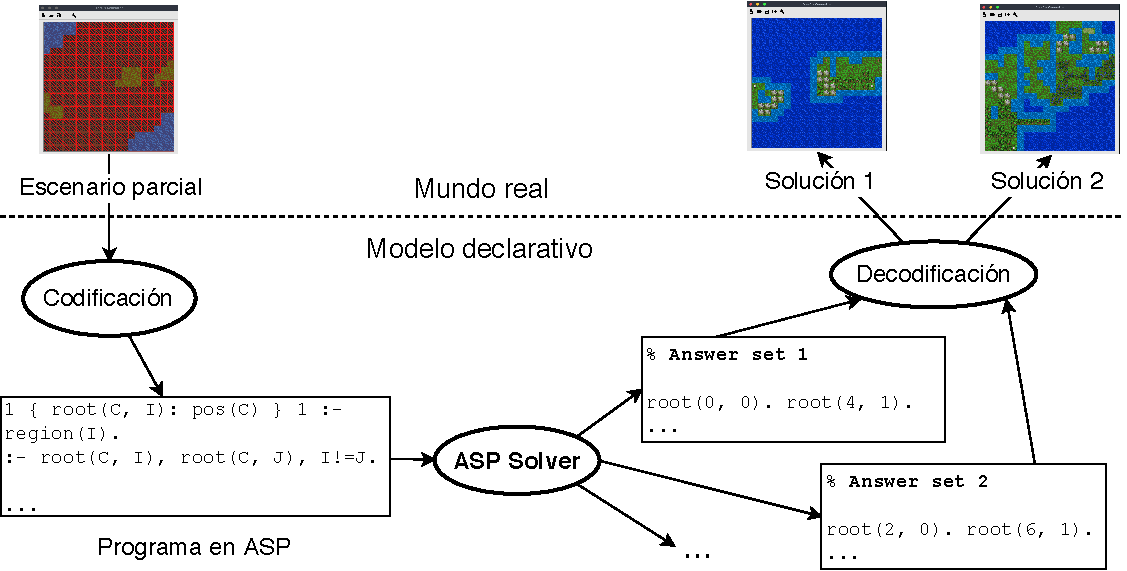
\includegraphics[width=0.9\textwidth]{images/funcionamiento-asp.pdf}
	
\end{frame}

\begin{frame}
\frametitle{Generación del escenario}

\begin{columns}
	\column{0.6\textwidth}
	\begin{itemize}
		\item<1-> Generar todo el terreno a la vez es \textcolor{UDCpink}{inviable}.
		
		\vspace{0.5em}
		
		\item<2-> Se divide el mapa en \textcolor{UDCpink}{cuadrantes} y \textcolor{UDCpink}{regiones}.
		
		\vspace{0.5em}
		
		\begin{itemize}
			\item<2-> Un cuadrante es un grupo de celdas
		\end{itemize}
		
		\begin{enumerate}
			\item<3-> Se genera regiones, que son grupos de cuadrantes conectados entre sí.
			
			\vspace{0.5em}
			
			\item<4-> Se detalla el terreno de cada región, formando islas.
		\end{enumerate}
		
		\vspace{0.5em}
		\item<5-> Los módulos son \textcolor{UDCpink}{independientes}. No necesitan toda la información del problema.
	\end{itemize}
	
	\column{0.4\textwidth}
	\centering
	\begin{overprint}
		\onslide<3>\centering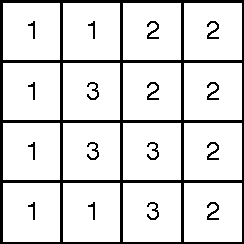
\includegraphics[width=0.9\textwidth]{images/regiones.pdf}
		\onslide<4-|handout:0>\centering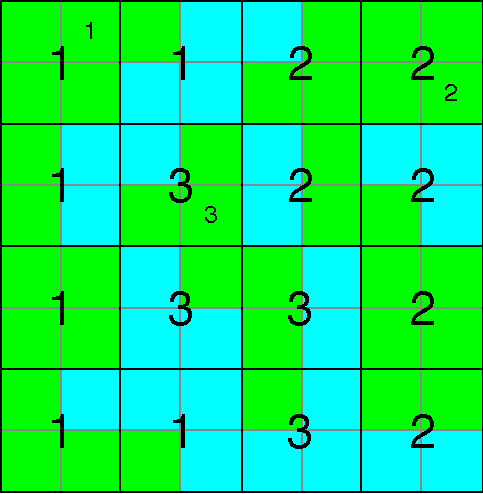
\includegraphics[width=0.9\textwidth]{images/celdas.pdf}
	\end{overprint}
\end{columns}
\end{frame}

\begin{frame}
\frametitle{Ejemplo de algunos predicados usados}

\begin{table}
	\def\arraystretch{1.5}
	\centering
	\begin{tabular}{l p{0.6\textwidth}}
		\hline
		\texttt{root(C, I)} & Cuadrante inicial \texttt{C} de la región \texttt{I}. \\
		\hline
		\texttt{pos(C)} & Posición \texttt{C} de un cuadrante. \\
		\hline
		\texttt{reached(C, I)} & Cuadrante \texttt{C} que ha sido alcanzado. \\
		\hline
		\texttt{adj(C, D)} & Posiciones adyacentes \texttt{C} y \texttt{D} en la cuadrícula. \\
		\hline
		\texttt{land(C)} & Celda \texttt{C} definida como tierra. \\
		\hline
		\texttt{mountain(C)} & Celda \texttt{C} definida como montaña. \\
		\hline
	\end{tabular}
\end{table}

\end{frame}

\begin{frame}
	\frametitle{Ejemplo de algunas reglas lógicas}
	
	\begin{block}{Generación del cuadrantes}		
	\vspace{1em}
	\hspace{2em}\texttt{reached(C, I) :- root(C, I).}
	
	\vspace{1em}
	
	\pause
	
	\hspace{2em}\texttt{0 \{ reached(C, I) \} 1 :- region(I), reached(D, I),}
	
	\hspace{4em}\texttt{adj(D, C), not existsanother(C, I).}
	
	\vspace{1em}
	
	\pause
	
	\hspace{2em}\texttt{1 \{ root(C, I): pos(C) \} 1 :- region(I).}
	
	\vspace{1em}
	
	\pause
	
	\hspace{2em}\texttt{:- root(C, I), root(C, J), region(I), region(J), I!=J.}
	\vspace{1em}
	\end{block}
	
\end{frame}

\begin{frame}
	\frametitle{Ejemplo de algunas reglas lógicas}

	\begin{columns}
	
	\column{0.6\textwidth}
	\begin{block}{\small Generación del cuadrantes}
		\small
		
		\vspace{1em}
		\hspace{1em}\texttt{reached(C, I) :- root(C, I).}
		
		\vspace{1em}
		
		\hspace{1em}\texttt{0 \{ reached(C, I) \} 1 :- }
		
		\hspace{3em}\texttt{region(I), reached(D, I),}
		
		\hspace{3em}\texttt{adj(D, C),}
		
		\hspace{3em}\texttt{not existsanother(C, I).}
		
		\vspace{1em}
		
		\hspace{1em}\texttt{1 \{ root(C, I): pos(C) \} 1 :-}
		
		\hspace{3em}\texttt{region(I).}
		
		\vspace{1em}
		
		\hspace{1em}\texttt{:- root(C, I), root(C, J),}
		
		\hspace{3em}\texttt{region(I), region(J), I!=J.}
		\vspace{1em}
	\end{block}
	
	\column{0.4\textwidth}
	\begin{overprint}
		\onslide<1>\centering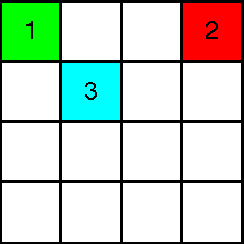
\includegraphics[width=0.9\textwidth]{images/expansion-1.pdf}
		\onslide<2|handout:0>\centering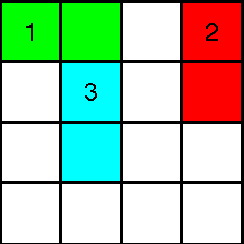
\includegraphics[width=0.9\textwidth]{images/expansion-2.pdf}
		\onslide<3|handout:0>\centering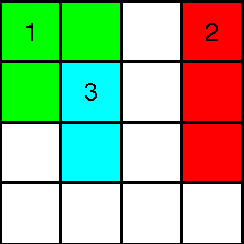
\includegraphics[width=0.9\textwidth]{images/expansion-3.pdf}
		\onslide<4|handout:0>\centering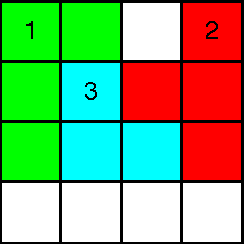
\includegraphics[width=0.9\textwidth]{images/expansion-4.pdf}
		\onslide<5|handout:0>\centering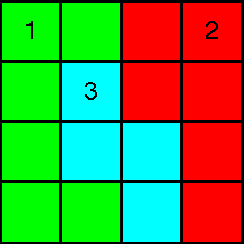
\includegraphics[width=0.9\textwidth]{images/expansion-5.pdf}
	\end{overprint}
	
	\end{columns}

\end{frame}

\begin{frame}
\frametitle{Generación de biomas y de puntos de inicio}

\begin{columns}
	\column{0.6\textwidth}
	
	\begin{itemize}
		\item<1-> \textcolor{UDCpink}{Generación de biomas}:
		
		\vspace{0.5em}
		
		\begin{itemize}
			\item<1-> Un bioma es una zona con el \textcolor{UDCpink}{mismo tipo de terreno}.
			
			\vspace{0.5em}
			
			\item<2-> Misma forma que la generación de islas, salvo que se pueden \textcolor{UDCpink}{pegar}.
		\end{itemize}
	\end{itemize}
	
	\column{0.4\textwidth}
	\centering
	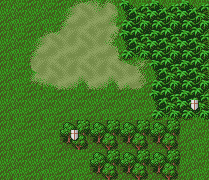
\includegraphics[width=0.6\textwidth]{images/biomas.png}
	
\end{columns}

\vspace{1em}

\begin{itemize}
	\item<3-> \textcolor{UDCpink}{Generación de puntos de inicio}:
	
	\vspace{0.5em}
	
	\begin{itemize}
		\item<3-> Se escoge N celdas de tierra para los jugadores.
		
		\vspace{0.5em}
		
		\item<4-> Para estos puntos se añaden preferencias:
		
		\vspace{0.5em}
		\begin{itemize}
			\item<4-> \textcolor{UDCpink}{Minimizar la distancia al agua}.
			
			\vspace{0.5em}
			
			\item<5-> \textcolor{UDCpink}{Maximizar la distancia a las montañas}.
		\end{itemize}
	\end{itemize}
\end{itemize}

\end{frame}